
%% bare_conf.tex
%% V1.4b
%% 2015/08/26
%% by Michael Shell
%% See:
%% http://www.michaelshell.org/
%% for current contact information.
%%
%% This is a skeleton file demonstrating the use of IEEEtran.cls
%% (requires IEEEtran.cls version 1.8b or later) with an IEEE
%% conference paper.
%%
%% Support sites:
%% http://www.michaelshell.org/tex/ieeetran/
%% http://www.ctan.org/pkg/ieeetran
%% and
%% http://www.ieee.org/

%%*************************************************************************
%% Legal Notice:
%% This code is offered as-is without any warranty either expressed or
%% implied; without even the implied warranty of MERCHANTABILITY or
%% FITNESS FOR A PARTICULAR PURPOSE!
%% User assumes all risk.
%% In no event shall the IEEE or any contributor to this code be liable for
%% any damages or losses, including, but not limited to, incidental,
%% consequential, or any other damages, resulting from the use or misuse
%% of any information contained here.
%%
%% All comments are the opinions of their respective authors and are not
%% necessarily endorsed by the IEEE.
%%
%% This work is distributed under the LaTeX Project Public License (LPPL)
%% ( http://www.latex-project.org/ ) version 1.3, and may be freely used,
%% distributed and modified. A copy of the LPPL, version 1.3, is included
%% in the base LaTeX documentation of all distributions of LaTeX released
%% 2003/12/01 or later.
%% Retain all contribution notices and credits.
%% ** Modified files should be clearly indicated as such, including  **
%% ** renaming them and changing author support contact information. **
%%*************************************************************************


% *** Authors should verify (and, if needed, correct) their LaTeX system  ***
% *** with the testflow diagnostic prior to trusting their LaTeX platform ***
% *** with production work. The IEEE's font choices and paper sizes can   ***
% *** trigger bugs that do not appear when using other class files.       ***                          ***
% The testflow support page is at:
% http://www.michaelshell.org/tex/testflow/



\documentclass[11pt]{IEEEtran}
% Some Computer Society conferences also require the compsoc mode option,
% but others use the standard conference format.
% If IEEEtran.cls has not been installed into the LaTeX system files,
% manually specify the path to it like:
% \documentclass[conference]{../sty/IEEEtran}



\usepackage{graphicx}
\usepackage[justification=centering]{caption}


% correct bad hyphenation here
\hyphenation{op-tical net-works semi-conduc-tor}


\begin{document}
%
% paper title
% Titles are generally capitalized except for words such as a, an, and, as,
% at, but, by, for, in, nor, of, on, or, the, to and up, which are usually
% not capitalized unless they are the first or last word of the title.
% Linebreaks \\ can be used within to get better formatting as desired.
% Do not put math or special symbols in the title.
\title{Localizing Sub-THz Curving Beam Transmitters with Multi-Frequency Modified Gerchberg-Saxton Phase Retrieval}


% author names and affiliations
% use a multiple column layout for up to three different
% affiliations
\author{\IEEEauthorblockN{Alan Chavez\\}
\IEEEauthorblockA{Rice University
}}

\maketitle


\IEEEpeerreviewmaketitle

\section{Introduction}

Curving beams have recently drawn significant interest due to their unique potential to mitigate blocking events in communications and sensing applications, including curving data links around obstacles in near-field sub-THz deployments\cite{CurvingData}.
The same property enables nonlocalizable jamming, where a jammer curves its beam around an obstacle so that the direction of arrival at the victim does not reveal the jammer's location\cite{spindel_jamming}.
In prior literature, the trajectory of such beams has been determined through two-dimensional spatial heatmaps of measured intensity\cite{AiryObservation, spindel_ms}.
This approach is impractical in real world settings, where complete spatial field measurements are unavailable.

Prior work showed in simulation and over-the-air (OTA) testing that a modified Gerchberg--Saxton (GS) phase retrieval algorithm can recover the phase profile at the transmit aperture of a caustic beam\cite{Froehly, beam_tutorial} from one dimensional receive measurements, provided the location and size of the transmit aperture are known.
In real jamming and communications scenarios, however, the location of the transmitter may not be known.
Localizing the transmitter itself from one dimensional measurements has not been explored.
To address this gap, the modified GS algorithm is wrapped in a grid search over speculative transmit aperture locations, with integrated multi-frequency support added so that multiple frequencies are solved for in a single run.
The localization error is quantified against receiver element spacing, bandwidth, and search grid resolution.

\section{Modified Gerchberg--Saxton Phase Retrieval}

The GS algorithm reconstructs a complex wavefront by propagating it forward and backward between the transmit and receive aperture planes while constraining the amplitude in each plane with measured values\cite{generic_mgs}.
After some amount of iterations the algorithm converges on a solution, which is not guaranteed to be unique\cite{generic_mgs}.
Prior work established the modifications that GS requires to function in the sub-THz regime, producing the modified GS (MGS) algorithm.
The Fraunhofer propagation model is replaced with Rayleigh-Sommerfeld, since meaningful measurements of sub-THz curving beams take place in the near-field region, at a cost of 3 Fast Fourier Transforms (FFT) per propagation instead of 1\cite{mmwave_phase_retrieval, rs_impl}.
The unconstrained phase iteration is replaced with gradient descent on a weighted mean square error (MSE) computed at the receive plane, weighted to favor the high amplitude regions where the signal-to-noise ratio (SNR) is highest\cite{mgs_descent}.
Lastly, phase as well as amplitude is measured at the receive aperture, which is pragmatic in the sub-THz regime but not available at optical frequencies.
MGS does not produce unique solutions, and requires prior knowledge of the geometry of the transmitter.
To solve this, MGS is paired with a grid search algorithm which exhaustively searches over possible transmitter locations and ranks the resulting candidates.
Multiple frequencies are also included in the solve, since curving beams bend differently at each frequency, providing additional constraints against non-unique solutions.

\section{Integrated Multi-Frequency Support}

Previously, multi-frequency measurements were exploited by running MGS once per frequency and averaging the results.
Instead, all measured frequencies are solved in a single MGS run, which further constrains the problem because each frequency bends slightly differently on its way to the receiver.
The solve is built around a center frequency, in this case 150 GHz, since that is reasonably achievable on the Rice Networks Group's KeySight testbed.
When bandwidth is added, a high frequency and a low frequency are added as constraints around the center: \(\pm\)1\% bandwidth, for example, corresponds to 148.5 GHz, 150 GHz, and 151.5 GHz.
All frequencies share one aperture profile.
This models a physical phase plate rather than an independent phase mask per frequency.
However, solving multiple frequencies at once introduces many more local minima that can trap the gradient descent in incorrect solutions.
In practice, a randomly initialized multi-frequency solve stalls roughly two orders of magnitude above the residual error floor that the same solver reaches when initialized well.
To avoid this, a warm start is used to initialize the solve.
MGS is first run on the center frequency alone, where the smoother single-frequency landscape reliably recovers the shape of the aperture profile.
The recovered phase is then unwrapped and used to initialize the multi-frequency iterations, which descend into the correct basin.
The warm start also sharpens localization: at the true transmitter location the residual error falls to the floor, while at candidate locations far from the transmitter no single aperture profile can reconcile the differing geometry across frequencies, so they fit the measurements poorly.
This contrast is the signal the grid search ranks on.

\section{Transmitter Localization via Grid Search}

Because phase retrieval requires the location of the transmit aperture to be known, localization is performed by wrapping MGS in an exhaustive search over a grid of speculative transmit aperture locations.
For each candidate location, MGS is run against the known one dimensional receive measurements, producing a candidate transmit aperture.
A grid search is convenient to implement, embarrassingly parallel, and requires no gradient information about the search space.
Therefore the grid search approach was adopted.
Candidates are ranked by the final residual error of their MGS solve.
A candidate placed far from the true transmitter produces a reconstruction that fits the receive measurements poorly, while a candidate near the true location reproduces the measured beam with a small residual error.
Since neighboring grid cells can produce nearly identical residual errors, the reported candidate set, referred to as the top candidates, is the 8-connected cluster of cells with residual error at most \(1.5\times\) the minimum, grown around the cell with the lowest residual error.
The size of this set is adaptive, and is reported as \(n\) alongside every result.
The mean distance of the top candidates from the true location is reported as the top candidates mean.

\section{Simulation Results}

The localization system is evaluated at two receiver element pitches, \(\lambda\)/20 and \(\lambda\)/2, where \(\lambda = 2.0\) mm at the 150 GHz center frequency, each across ten bandwidth settings, and the sensitivity of the results to the search grid resolution is then tested.

\subsection{Simulation Setup}

As in the prior work, the simulated scenario mimics what the Rice Networks Group's KeySight testbed can reasonably accomplish.
The true transmit aperture is centered at \(z = 0.30\) m with the one dimensional receive aperture on the \(z = 0\) axis, and the center frequency is 150 GHz.
Each speculative candidate assumes a 100 mm wide transmit aperture.
Bandwidth is swept as \(\pm\)\{0, 1, 2, 3, 5, 7, 10, 13, 16, 20\}\% of 150 GHz, where 0 denotes a single tone.
The search grid covers \(z \in [0.15, 0.80]\) m and \(x \in [-0.15, 0.15]\) m with \(164 \times 76 = 12{,}464\) candidate locations, giving cells approximately 4.0 mm square, or about \(2\lambda\), so the best achievable candidate sits 1.83 mm from the true location.
The base of the beam is approximately 50 mm wide.
The conditions are deliberately idealized: there is no noise, the SNR is unrealistically high, and the receive aperture captures 83.3\% of the beam's energy.
Figure \ref{fig:true_scene} shows the true beam, the aperture locations, and the MGS reconstruction when the transmitter location is known.

\begin{figure}[]
    \centering
    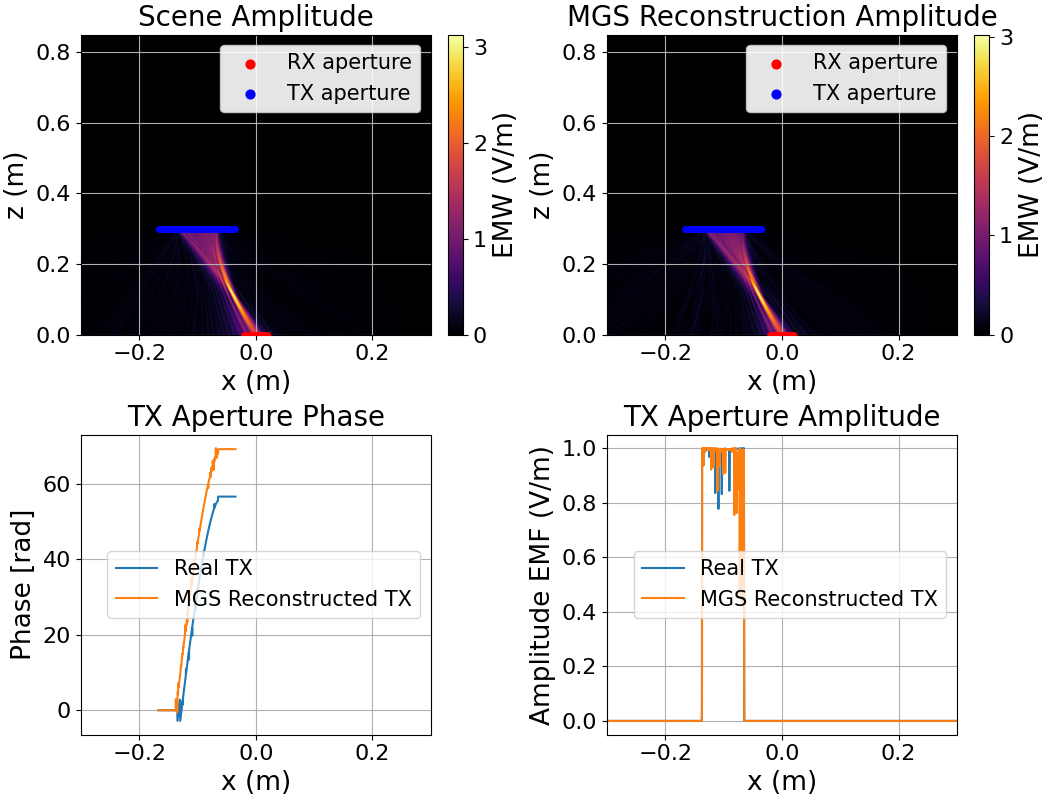
\includegraphics[width=1.0\linewidth]{true_mgs_scene.png}
    \caption{True Beam Scene and Known-Location MGS Reconstruction}
    \label{fig:true_scene}
\end{figure}

\subsection{\(\lambda\)/20 Receiver Results}

Figure \ref{fig:l20_1f} shows the candidate residual map for the \(\lambda\)/20 receiver with a single tone.
The residual error forms a deep, sharply defined basin: the candidate with the lowest residual error, \(3.1 \cdot 10^{-6}\), sits 11.81 mm from the true transmitter, with \(n = 11\) top candidates clustered near the true location.
Across the bandwidth sweep the candidate with the lowest residual error lands between 11.81 mm and 20.81 mm from the true location, with the largest errors at \(\pm\)2\% (18.27 mm) and \(\pm\)3\% (20.81 mm).
At every bandwidth of \(\pm\)5\% and above, the candidate with the lowest residual error is the same grid cell, 15.16 mm from the true location.
The top candidates mean ranges from 15.32 mm to 19.18 mm.
At this receiver pitch, adding bandwidth does not materially improve localization: a single tone already performs as well as any wider setting, and the error settles at a floor of approximately 15 mm.

\begin{figure}[]
    \centering
    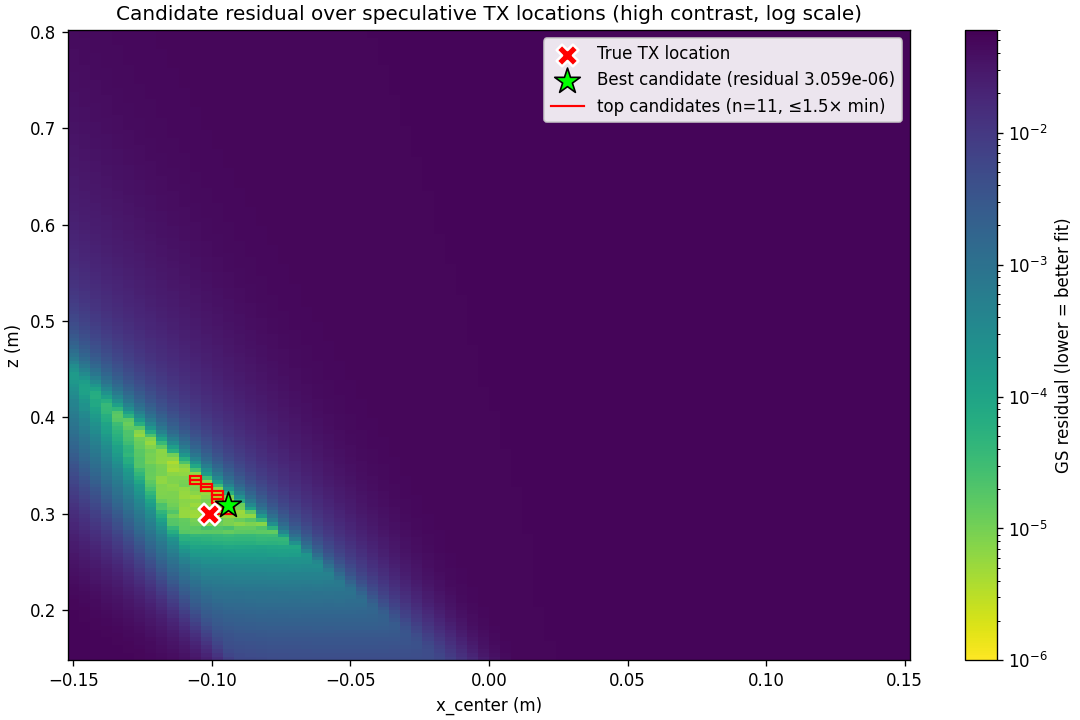
\includegraphics[width=1.0\linewidth]{heat_lambda20_1f.png}
    \caption{Candidate Residual Map \(\lambda\)/20 Single Tone}
    \label{fig:l20_1f}
\end{figure}

\subsection{\(\lambda\)/2 Receiver Results}

Figure \ref{fig:l2_1f} shows the residual map when the receiver element pitch is coarsened to \(\lambda\)/2.
With a single tone the candidate with the lowest residual error again lands 11.81 mm from the true location, but the basin is nearly flat: the top candidates cluster grows to \(n = 304\) cells with a mean distance of 41.51 mm, and the residual error basin is roughly \(36\times\) shallower, with a best residual error of \(1.1 \cdot 10^{-4}\).
Adding bandwidth concentrates the candidate set without restoring accuracy.
Figure \ref{fig:l2_pm10} shows the \(\pm\)10\% case, where \(n\) falls to 23, and \(n\) reaches 3 at \(\pm\)13\% and \(\pm\)16\%.
However, for 9 of 10 bandwidths the candidate with the lowest residual error is the same grid cell, 21.67 mm from the true location.
The top candidates mean never falls below 16.62 mm at any bandwidth.
At this receiver pitch, adding bandwidth reduces the ambiguity between candidates, but the error settles at a bias of approximately 21.7 mm.

\begin{figure}[]
    \centering
    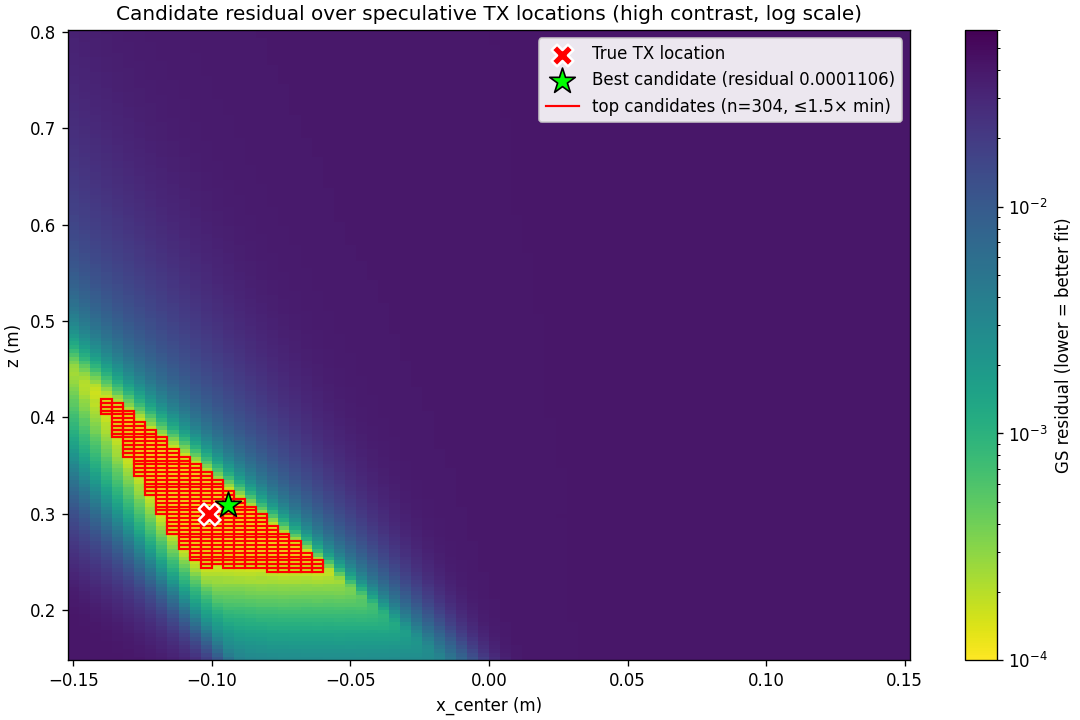
\includegraphics[width=1.0\linewidth]{heat_lambda2_1f.png}
    \caption{Candidate Residual Map \(\lambda\)/2 Single Tone}
    \label{fig:l2_1f}
\end{figure}

\begin{figure}[]
    \centering
    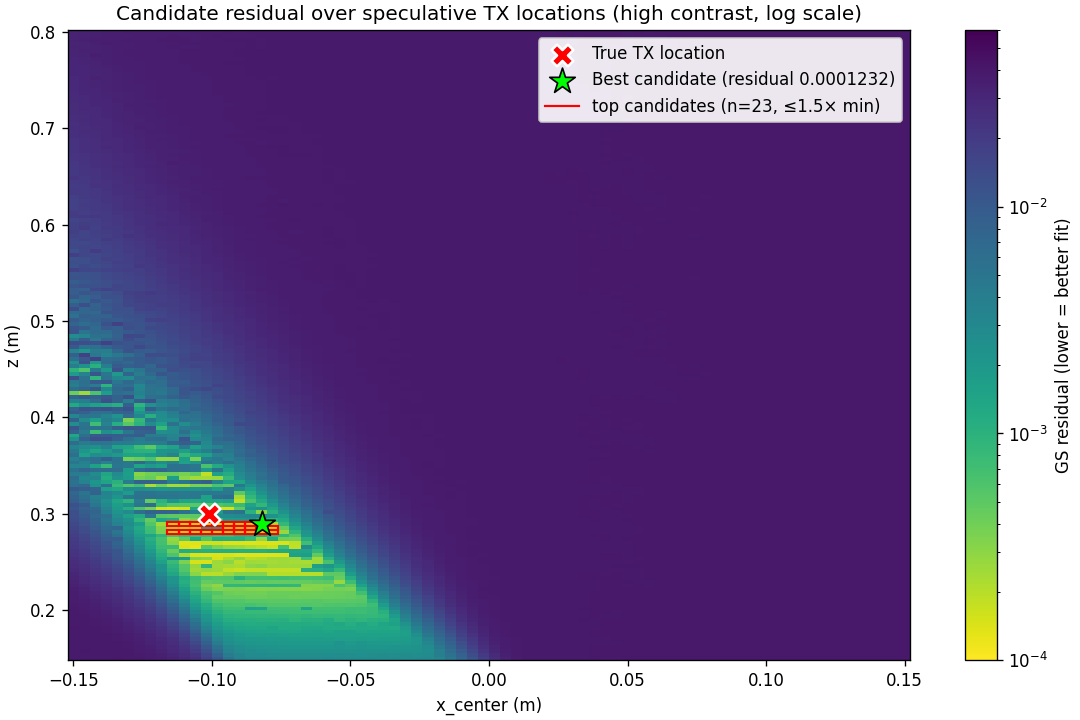
\includegraphics[width=1.0\linewidth]{heat_lambda2_pm10.png}
    \caption{Candidate Residual Map \(\lambda\)/2 \(\pm\)10\% Bandwidth}
    \label{fig:l2_pm10}
\end{figure}

\subsection{Grid Refinement Robustness Check}

The studies above were first run on a coarser \(64 \times 48\) search grid with 3,072 candidates and cells of \(10.32 \times 6.38\) mm.
At that cell size, errors below roughly 1.5 cells, about half a cell of pure quantization plus a cell of slack for ties between neighbors, could be explained by grid quantization rather than by the method itself.
To test this explanation, both studies were re-run on the \(164 \times 76\) grid.
If quantization explained the error floor, the errors should have shrunk with the cells.
They did not.

Figure \ref{fig:refine} shows the comparison for both receivers.
At \(\lambda\)/20, averaged across the bandwidth sweep, the candidate with the lowest residual error moved from 12.61 mm to 15.44 mm from the true location.
The top candidates mean rose from 10.52 mm to 17.38 mm.
The errors rose rather than shrank because the coarse lattice happened to place cells close to this particular true location, understating the bias that the finer grid then exposed.
At \(\lambda\)/2, the candidate with the lowest residual error landed erratically on the coarse grid, between 9.70 mm and 46.87 mm from the true location.
On the refined grid it settled onto the stable 21.67 mm bias, and the apparent bandwidth improvements in the top candidates mean, such as 7.44 mm at \(\pm\)5\%, vanished entirely.
Figure \ref{fig:pitch_cmp} shows both receivers on the refined grid.

Ranking all candidates by residual error gives the same picture.
At \(\lambda\)/20 with a single tone, the cell nearest the true location ranks 33rd of 12,464 candidates, in the top 0.26\%.
On the coarse grid its rank was 7th of 3,072, essentially the same percentile, so the refinement mostly inserted near-ties without reshaping the residual error basin.
At \(\lambda\)/2, the cell nearest the true location falls from the top 0.37\% at a single tone to the 7.5th percentile at \(\pm\)20\%, so the ranking is systematically biased away from the true location.

The refinement therefore removed the quantization explanation, exposing a real error floor of approximately 15 mm at \(\lambda\)/20 and a stable 21.7 mm bias at \(\lambda\)/2 that bandwidth does not remove.
The remaining error floor is likely dominated by the geometry of the aperture itself.
Each candidate assumes a 100 mm wide aperture, but the beam leaving it is only about 50 mm, or \(25\lambda\), wide.
Since the beam does not fill the aperture, multiple aperture placements can faithfully reconstruct the same beam, and the residual error cannot separate them.

\begin{figure}[]
    \centering
    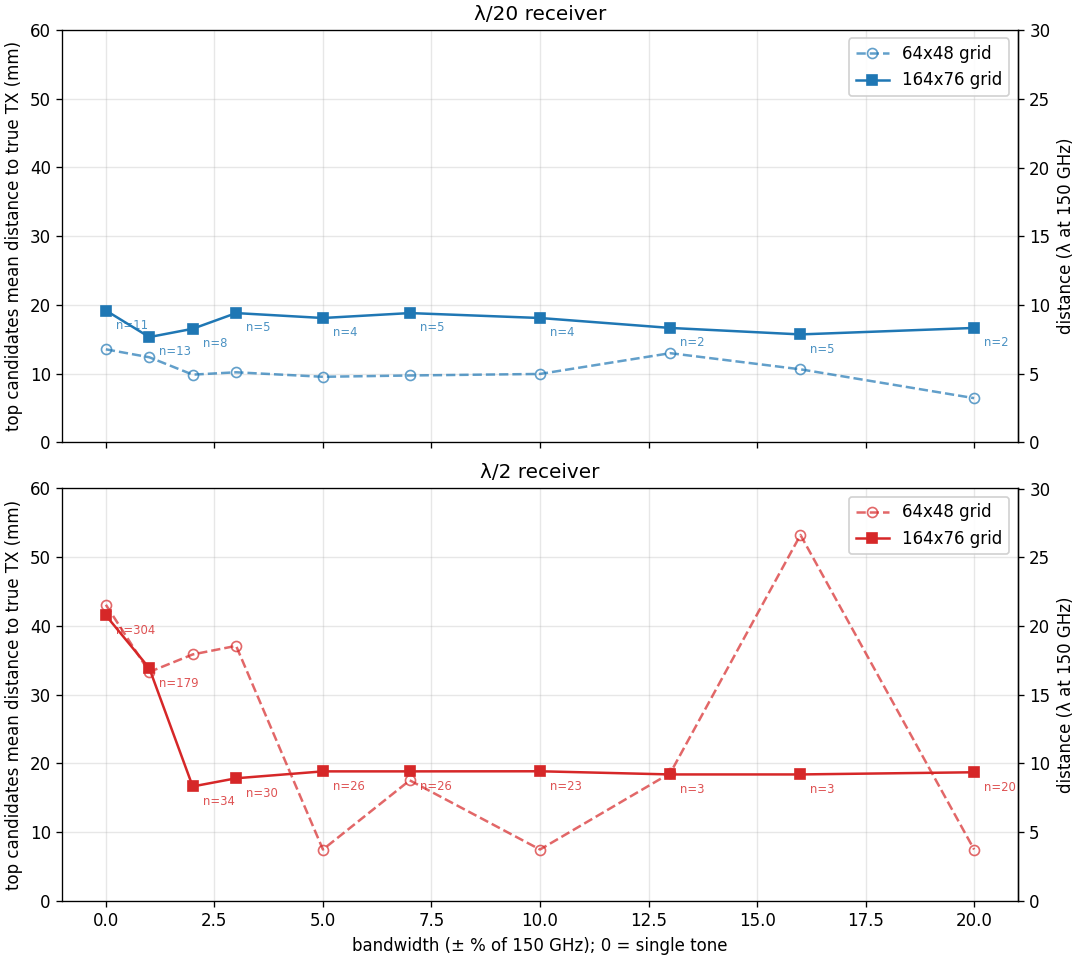
\includegraphics[width=1.0\linewidth]{error_coarse_vs_fine.png}
    \caption{Grid Refinement Comparison}
    \label{fig:refine}
\end{figure}

\begin{figure}[]
    \centering
    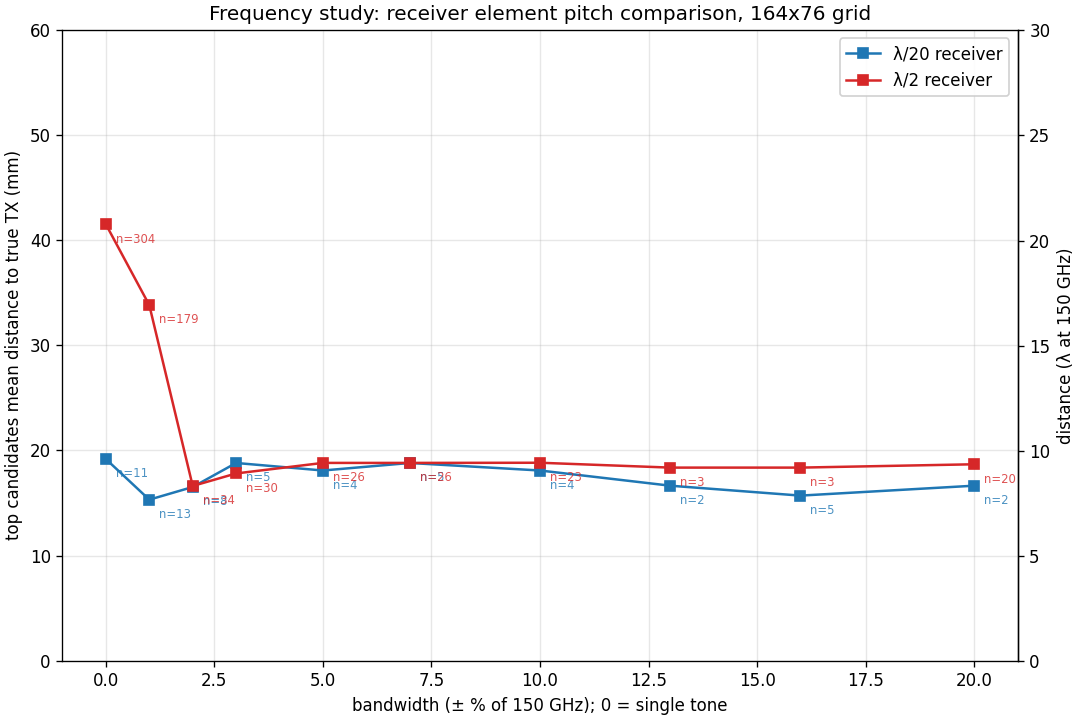
\includegraphics[width=1.0\linewidth]{error_vs_bw_pitch.png}
    \caption{Receiver Element Pitch Comparison \(164 \times 76\) Grid}
    \label{fig:pitch_cmp}
\end{figure}

\section{Limitations of Proposed Approach}

The reported results are a best case.
There is no noise, the SNR is unrealistically high, and the receive aperture captures the large majority of the beam's energy.
Under realistic receiver noise the value of frequency diversity measured here is likely an underestimate, since the near-ties that bandwidth serves to disambiguate would otherwise be dominated by noise.

Furthermore, all results come from a single scenario with one true transmitter location, trajectory, and geometry, so the error floor may not generalize to other scenes.
The search additionally assumes the width of the transmit aperture is known, inheriting the prior work's requirement.

The localization error is also measured from the center of the candidate aperture to the center of the true aperture.
Since multiple aperture placements can carry the same beam, some of the reported error may be noise added by the metric rather than a failure to recover the beam, and a metric defined on the beam itself may be fairer.

The computation cost remains extraordinary.
Each study point requires 12,464 full MGS solves and takes a long time to complete even when fully parallelized.
These computation limits make the approach infeasible for real time localization of an active transmitter, and the cost scales directly with the number of candidate locations searched.

Lastly, at \(\lambda\)/2 pitch the ranking itself becomes ambiguous.
The adaptive top candidates cluster reaches \(n = 304\) tied cells at a single tone, so reporting a single answer requires an arbitrary tie-break, and defining the boundary of the candidate region is itself ambiguous.
No OTA validation of the localization system has been performed, so all results remain simulation.

\section{Conclusion}

A methodology for localizing a sub-THz curving beam transmitter from one dimensional receive measurements was demonstrated, wrapping a modified Gerchberg--Saxton phase retrieval algorithm in a grid search over speculative transmitter locations with integrated multi-frequency support.
At \(\lambda\)/20 receiver spacing, a single tone localized the transmitter to within 12 mm of the true location, and the error remained near 15 mm across the bandwidth sweep.
At \(\lambda\)/2 spacing, localization degraded to a stable 21.7 mm bias that additional bandwidth did not remove.

Refining the search grid falsified the quantization explanation for the localization error, exposing a floor of approximately 15 mm at \(\lambda\)/20, and showed that under the idealized conditions tested, frequency diversity was not needed.
Despite these limits, the proposed approach offers a promising pathway toward localizing curving beam transmitters in scenarios where conventional field-mapping techniques are impractical.
Future work will focus on validating the system over the air under realistic receiver noise, and on determining whether the remaining error floor is caused by the assumed transmitter aperture geometry.



% conference papers do not normally have an appendix


% trigger a \newpage just before the given reference
% number - used to balance the columns on the last page
% adjust value as needed - may need to be readjusted if
% the document is modified later
%\IEEEtriggeratref{8}
% The "triggered" command can be changed if desired:
%\IEEEtriggercmd{\enlargethispage{-5in}}

% references section

\bibliographystyle{plain}
\bibliography{main}



% that's all folks
\end{document}
